\documentclass[11pt]{article}
\usepackage[a4paper, margin=1in]{geometry}
\usepackage[french]{babel}
\usepackage{graphicx}
\usepackage{epstopdf}
\usepackage{tabularx}
\usepackage{float}
\usepackage{hyperref}
\usepackage{pdfpages}

\begin{document}
\pagestyle{empty}

\begin{titlepage}
\begin{flushright}
    \textit{Roselies, le \today }
\end{flushright}

\begin{minipage}{0.5\textwidth}
\begin{flushleft}
    \textbf{\LARGE MATHIEU Raphael} \\
    Ingénieur Géomètre GEO21/1547 \\
    \vspace{3mm}
    Rue J. Wauters 52\\
    6250 Roselies \\
    \vspace{3mm}
    Email: \href{mailto:mathieu.geometre@gmail.com}{mathieu.geometre@gmail.com}\\
    GSM: \href{tel:+32471784815}{0471/78.48.15} \\
\end{flushleft}
\end{minipage}
\hfill
\begin{minipage}{0.5\textwidth}
\begin{flushright}
    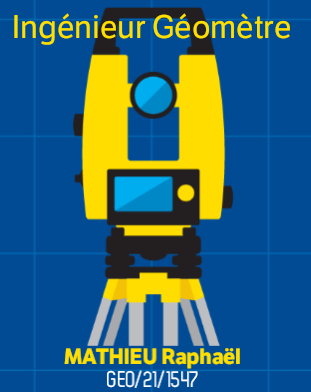
\includegraphics[scale=0.4]{"D:/Pharmacy_Raph/Codes/LogoGeometre.png"}  
\end{flushright}
\end{minipage}

\vspace{10mm}

\hrule

\begin{center}
    \huge\textbf{Objet : Demande de transfert de pharmacie}\\
    \vspace{2mm}
    \huge\textbf{{{ Name_pharma }} (APB {{ Id_pharma }})} \\
\end{center}
\vspace{35mm}
\includegraphics[width=\textwidth]{{{ Map_new_implentation }}}

\end{titlepage}



\clearpage% Body
\begin{center}
    \section*{\Huge Demande de transfert}
\end{center}

\vspace{10mm}

Rapport de transfert de la {{ Name_pharma }} (N° APB {{ Id_pharma }}) depuis {{ Old_adress }}- {{ Old_postcode }} {{ Old_town }} vers {{ New_adress }} - {{ New_postcode }} {{ New_town }}.

\vspace{25mm}

\section*{Coordonnées Lambert 2008}
\begin{minipage}{0.5\linewidth}
Adresse actuelle: \\
X : {{ Old_X }} m \\
Y : {{ Old_Y }} m \\
\end{minipage}
\hfill
\begin{minipage}{0.5\linewidth}
    Nouvelle adresse:\\
    X : {{ New_X }} m\\
    Y : {{ New_Y }} m\\
\end{minipage}

\vspace{10mm}

\section*{Distance entre les deux adresses}
% \begin{figure}[H]
%     \centering
%     \includegraphics[width=0.6\textwidth]{example-image}
%     \caption{\textit{Extrait du plan "Distance entre les deux adresses" du {{ Date_plan }} - réf : {{ Ref_dossier }}. Plan en annexe 1 de ce document }} 
% \end{figure}


\noindent Distance totale entre les deux adresses par la voie publique : {{ Distance_road }} m\\

\noindent Distance "à vol d'oiseau" : {{ Distance_fly }} m\\

\vspace{25mm}
\noindent \textbf{\large J'atteste par la présente que la pharmacie se déplace bien dans un rayon de 3000m.}\\

\vspace{25mm}

\noindent Rapport rédigé par MATHIEU Raphaël, Ingénieur géomètre, légalement admis et assermenté en cette qualité par le Tribunal de première Instance séant à Namur, inscrit au Conseil Fédéral des géomètres-experts sous le numéro GEO/21/1547.
\vspace{10mm}
\begin{flushright}
    \textit{Rapport établi à Aiseau-Presles le \today }
\end{flushright}

\clearpage
\include{table_new_implentation}

\clearpage
\include{table_old_implentation}

\includepdf[fitpaper,rotateoversize]{{{ Map_new_implentation }}}

\includepdf[fitpaper,rotateoversize]{{{ Map_all_itinerary_new }}}

\includepdf[fitpaper,rotateoversize]{{{ Map_all_itinerary_old }}}

\end{document}